\documentclass[11pt]{article}
\usepackage[margin=2cm]{geometry}
\usepackage{setspace}
\doublespacing
\usepackage{lineno}
\usepackage{graphicx}
\usepackage{float}
\usepackage{siunitx}


\title{
CMEE miniproject \\
\textbf{ Model selection on the abundance of freshwater microbial under the condition of global warming}}
\author{Yuxin Qin }
\date{Mar 2019}

\begin{document}
\maketitle

\begin{center}
Department of life sciences (Silwood Park)\\
Imperial College London  \\
\bigbreak
yq3018@imperial.ac.uk
\bigbreak
\bigbreak
\bigbreak
\bigbreak
\bigbreak
\bigbreak
Word Count: 2503
\end{center}

\newpage

\begin{linenumbers}
\section*{Abstract}
The increasing temperature of earth has threaten the freshwater microbial communities due to the vulnerability and temperature dependancy of freshwater system. Reduced bodysize is a key biological response to the warming condition in many ectothermic taxa for it has significant influence on the life history and metabolic mechanism. Both Yvon and Stewart did similar mesocosm experiments to test the impact of warming condition on freshwater microbial communities, but they came to different conclusions. Yvon claimed that community biomass declined significantly under warming condition and the slope of log(abundance) against log(bodysize) in warming condition was steeper. While Stewart's experiment cannot prove the statement of Yvon.
The aim of this article was to reanalyze Stewart's data and compare the allometric scaling model and the Plante-Downing model. It turned out that the Plante-Downing model performed better than the allometric scaling model in Akaike information criterion (AIC), but the allometric scaling model also gave us valuable information on understanding the impacts of global warming on freshwater microbial communities. Other results had shown to consist with Yvon's statement.



\section*{Introduction}
According to the IPCC report published in 2018, the surface temperature of earth has incresed approximately \SI{1.0}{\celsius} compared to pre-industrial levels and it tends to reach \SI{1.5}{\celsius} between 2030 and 2052 if the current rate of global warming continues in the following years \cite{IPCC}.
Since the phrase global warming first appeared in 1957, many scientists have studied the impacts of global warming in differnt scales and different organisms like climate change, crop production, coral bleach and so on \cite{weart2009discovery}.
Due to the vulnerability, temperature dependancy and the long term exposure to environmental stressors, it is significant to study the impacts of global warming on freshwater system \cite{arnell1996effects}.
Previously, the study of global warming on freshwater system mainly focuesed on the distribution of freshwater and the potential changes of freshwater fish \cite{carpenter1992global},
but recently several studies discovered that warming has significant impacts on freshwater microbial communities via mesocosm experiemnts. \\
Utilizing mesocosm experiments to examine the impacts of warming on freshwater microbial communities allows researchers to control the key factor temperature between the experiment groups and the control groups.
Besides, mesocosm experiments also provide freshwater microbial communities with a more natural environment compared to laboratory experiments. Via the establishment mesocosm expeiments, Yvon discovered that warming significantly reduced the total freshwater microbial community biomass and significantly increased the steepness of the slope of community size spectrum \cite{yvon2011warming}.
Rebeca Stewart from University of London did a similar mesocosm experiment as Yvon during her phd, but she got different conclusion. She claimed that warming had no significant impact on freshwater microbial community biomass and warming did not significantly increased the steepness of the slope of community size spectrum \cite{rebecca}.
In order to clear the impacts of warming on freshwater microbial communities, I decided to reanalyze Stewart's data. \\
Here is a brief introduction on Stewart's mesocosm experiment setup and the collection method of required data.
The mesocosm experiment consisted of 2 groups of ponds, the control group and the experiment group. Each group had 10 outdoor, artificial ponds with the ability to hold approximately \( 1 m^3\) water.
The water in experiment ponds were warmed between 3-5 \SI{1.0}{\celsius} by electronic heating elements.
The experiment ponds and the control ponds were arranged randomly in the block design.
The biota seeded in the mesocosms were from the river Frome, Dorset, UK, containing 5 main groups of microbes, ciliate, algae, meiofauna, flagellate and heterothrophic protists.
These microbes were seeded to the ponds 10 months prior to the warming for further natual colonisation. The sample of microbial communities was performed monthly from February 2009 to January 2010.
10 ml water was removed from each pond using a sterile syringe at three depths of the pond, the water surface, the middle water column and the sediment surfae.
After the collection of samples, 1 ml subsample was removed from each sterile syringe and transferred to a 1 ml Sedgwich-Rafter counting cell for further data collection using light microscopy.
Stewart identified the group, family, genus, species and feeding type of each microbial individual in subsample and recorded its shape lively under microscopy.
She also measured the length and width of each microbial individual containing in the 1 ml subsample using image analysis software ImageJ and Q capture.
Therefore, the biovolume, abundance and biomass of each species or groups can be generated from the original data. \\
The objective of this article is to analyze the relationship of abundance, bodymass and biomass in freshwater microbial communities under warming condition.
Shrinking bodysize has been a severe ecological response to climate change and has been observed in a wide range of ectothermic taxa \cite{walters2006temperature}.
Bodysize is regarded as a key ecological feature for many biological characteristics  like reproduction, population density and growth rate, which are in allometric scaliing relationship with bodysize \cite{peters1983effect}.
The allometric scaling of bodysize and biological characteristic is a general law used in many systems including freshwater system \cite{yvon2011warming}.
Another model called Plante-Downing model is an empirical model with good prediction on the invertebrate population in freshwater system\cite{plante1989production}.
I intend to fit the freshwater microbial data collected by Stewart into the two models to evaluate coinfidence of the two models by Akaike information criterion (AIC).

\section*{Methods}
\section*{1 Data handling}
The data used in this article is based on the thesis of Rebecca stewart.
Due to some mistakes of the original datasheet, I refilled some blank space in temperature, deleted some abnormal data and recalculated the biovolume, bodymass and biomass of each data recorded.
Biovolume of each freshwater microbial was calculated from the length and width measured under the microscopy according to the shape recorded.
The equations used to calulate the biovolume followed the paper of Hillerbrand's paper\cite{hillebrand1999biovolume}.
Bodymass here refered to the individual mass, calculated by the equation $Bodymass = Biovolume * 0.14 * 1.1 $ according to Julia Resis's paper \cite{reiss2008existing}.
Biomass here refered to the carbon dry mass of a freshwater taxa, which was calculated by the mutiplication of 0.25 bodymass and abundance.
Meanwhile, I used dpply to reorganized the data for the convenience of fitting models.
\section*{2 Fitting model}
The models used to fit the abundance and bodymass are the allometric scaling model and the Plante-Downing model. The two model will be explained separately.
I compared the coinfidence of the two model by Akaike information criterion (AIC). The way to calculte the AIC of each model will also be explained later.   \\
\textbf{2.1 Allometric scaling model} \\
The allometric scaling model is shown below, where $y$ is the characteristic of interest, $x$ is bodysize. $a$ and $b$ here are constant.
The constant $a$ can be considered as the ratio of specific growth rate of $y$ and $x$ \cite{huxley1950relative}.
In the circumstance of my data, I put abundance as the biological characteristic $y$ and bodymass as the individual bodysize $x$.
In order to better fit the model, I log both bodymass and abundance.
The slope of this linear model can indicate the growth rate of bodymass and abundance.
\begin{equation}
     y= b x^a
\end{equation}
\textbf{2.2 Plante-Downing model} \\
The Plante-Downing model is an empirical model shown below, where $P$ is the population of freshwater invertebrate, $\overline{B}$ is the annual mean population biomass, $\mathit{W}_{m}$ is the maximum individual bodymass and $T$ is the ambient surface temperature \cite{plante1989production}.
This model has been proved to fit freshwater invetebrate communities quite well annually \cite{plante1989production}.
In my circumstance, I fit the model monthly and regard replace $P$ in the original formula with abundance. The rest parameters were performed as the original ones.
\begin{equation}
     \log(P) = a +b \log(\overline{B}) - c \log(\mathit{W}_{m}) + d T
\end{equation}
\textbf{2.3 Model selection} \\
To compare the two models, I used Akaike information criterion (AIC).AIC utilized the Kullback-Leibler information lost to measure the discrepancy between the true model and the approximating model \cite{wagenmakers2004aic}. The calculation of AIC is based on the Johnson's papaer \cite{johnson2004model}. I chose to use normal AIC becuase neither the number of free parameter $p$ in two selected models exceed $n/40$ (n is the sample size).As the sample size of the data is 4271,  $n/40 =4271/40 = 106.67 $. The number of free parameter in allometric model is 2 and the number of free parameter in Plante-Downing model is 4. Obviously, both 2 and 4 is smaller than the 106.67. Therefore, model selection in this case has no need to use the second order deriative of AIC, the $\mathit{AIC}_{c}$, which normally used to correct small sample size. \\
The formula to calculate AIC is shown below. In this formula, $L(\hat{\theta}|y)$ is the likelihood of the model parameters given the data. For models fitted by least squares with the usual assumptions,
$L(\hat{\theta}|y)=-n/2\ln(RSS/n)$. RSS here is the residual sum of squares for a linear model and n is the sample size.
\begin{equation}
AIC = -2 \ln [ L (\hat{\theta}|y)] + 2 p = -2 \ln [-n/2\ln(RSS/n)] + 2 p
\end{equation}

\section*{3 Computing languages}
The major languages used in the miniproject are bash and R. Bash was used to run the workflow like creating the report in LaTeX and running the R script. The calculation of data, model fitting and plotting are all performed in R version 3.2.3 (2015-12-10). There are several reasons that I chose R instead of python. One important reason allow me to choose R is the size of raw data only occupying 7.4Mb. Nevertheless, the calulation and model fitting in this miniproject are not too complex and  they are able to be handled by R very quickly. Moreover, R can provide a better visulisation than python on the plots. \\
The model fitting in this article was done by lm in R. The plots are produced by ggplot2 basically. I wrote some functions to generate the multi-plot, coefficient table and AIC table automatically with the gridExtra package and lappy.

\section*{Results}
\section*{1 Community biomass}
According to figure 1, we can know that the mean community biomass under warming condition is smaller than the one under cold or ambient condition, which is consistent with Yvon's conclusion.
\begin{figure}[H]
  \centering
  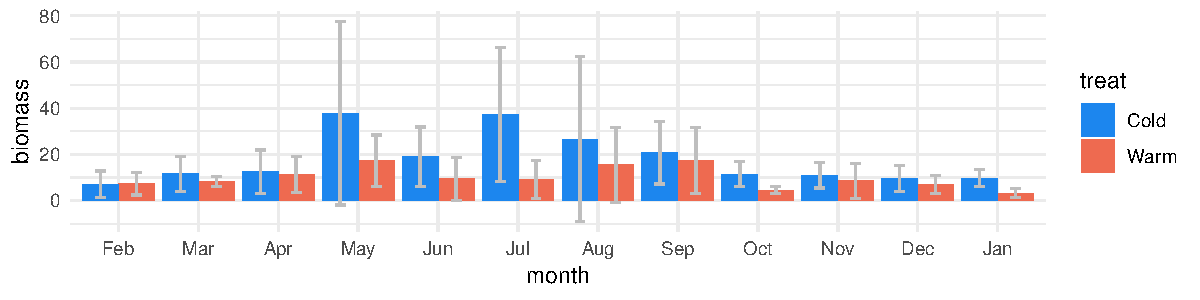
\includegraphics[scale = 0.8]{../Graph/CommunityBiomassPlot.png}
  \caption{\textbf{The mean community biomass in each month.}  }
\end{figure}

\section*{2 Allometric scaling model}
The coefficients of allometric scaling model under different conditions were listed in figure 2.
By plotting the slope of warming condition and ambient condition on the same graph as figure 3, we discovered that the slope of ambient condition is higher than the warming condition except for the first experiment month.
The slope of the linear model is also the coefficient of $log(bodymass)$, indicating a higher growth rate in population in the ambient condition compared to warming condition. These results support the conclusion driven by Yvon.
The bodysize of ectothermic taxa mainly determined by two ecological factors, nutrient supply and metabolic rate \cite{sheridan2011shrinking}. Since the nutrient supply is the same among all mesocosm ponds here, the reduction of bodymass in warming condition is likely to blame the decreasing metabolic rate. Figure 3 implicated that one potential consequence of rising temperature is the decline of metabolic rate among freshwater microbial communities.  \\
When we looked at figure 4 for the linear regression graph of allometric scaling model and the figure 5 for observed value against predicted value of $log(abundance)$, it was obvious that the data didn't fit well into the model.
\begin{figure}[H]
  \centering
  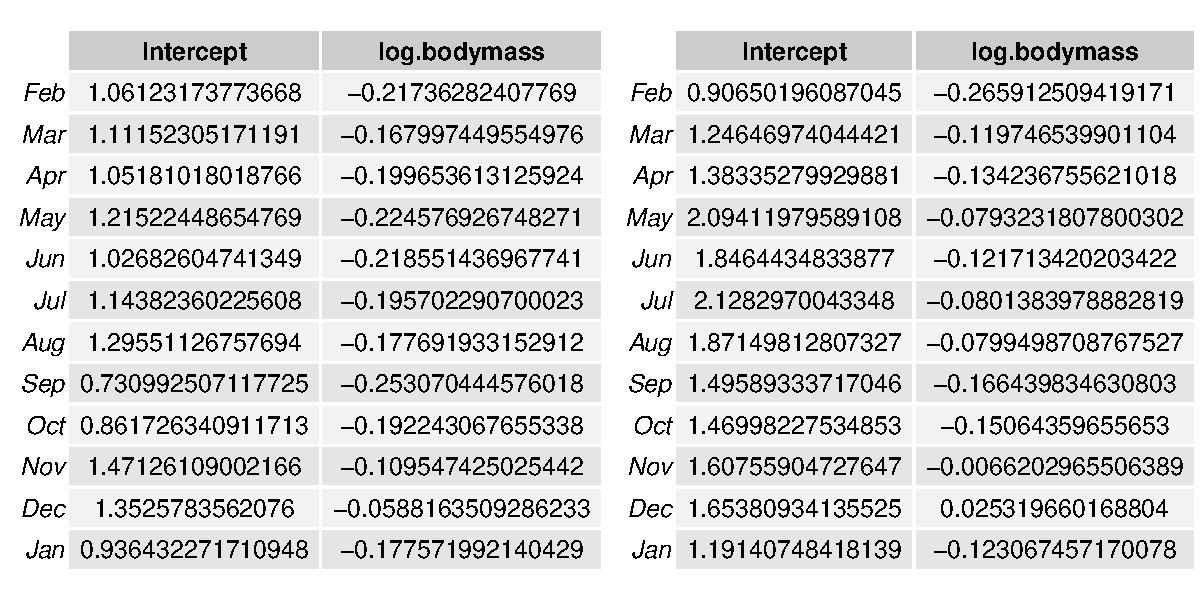
\includegraphics[scale = 0.8]{../Graph/ascoef.png}
  \caption{\textbf{The coefficients of the allometric scaling model.}  The table on the left is the coefficients under warm condition. The table in the right is the coefficients under ambient condition. }
\end{figure}

\begin{figure}[H]
  \centering
  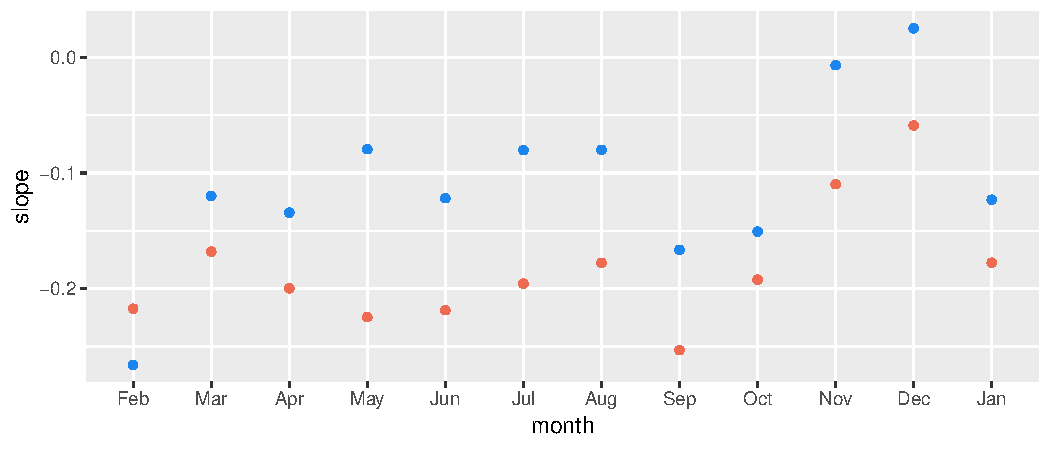
\includegraphics[scale = 0.8]{../Graph/ascoefplot.png}
  \caption{\textbf{The slope of allometric scaling model in each month.}  The red colour in graph represents samples of warming condition and the blue colour represents samples of ambient condition. }
\end{figure}

\begin{figure}[H]
  \centering
  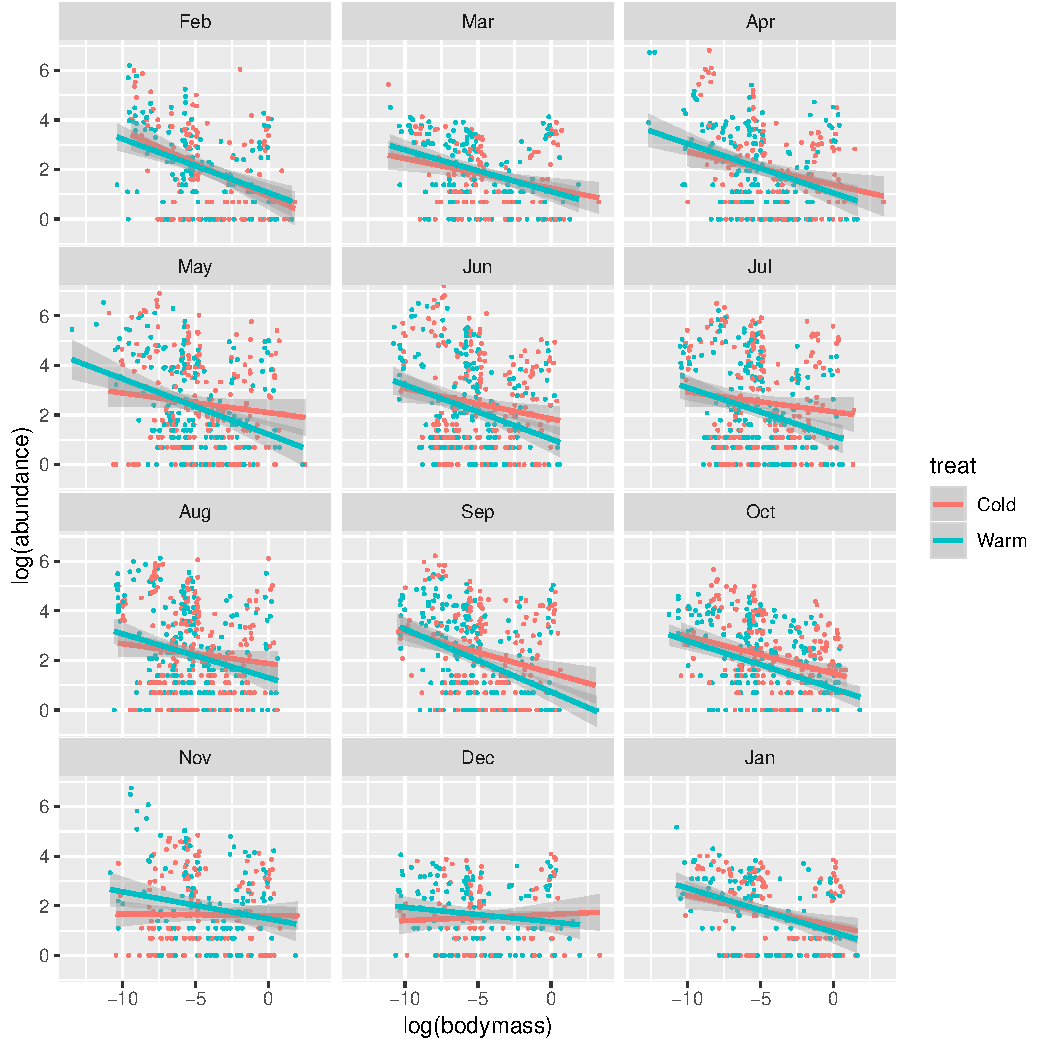
\includegraphics[scale = 0.5]{../Graph/as12l.png}
  \caption{\textbf{Linear regression graph of the allometric scaling model.}
  The red colour in graph represents samples of warming condition and the blue colour represents samples of ambient condition. }
\end{figure}

\begin{figure}[H]
  \centering
  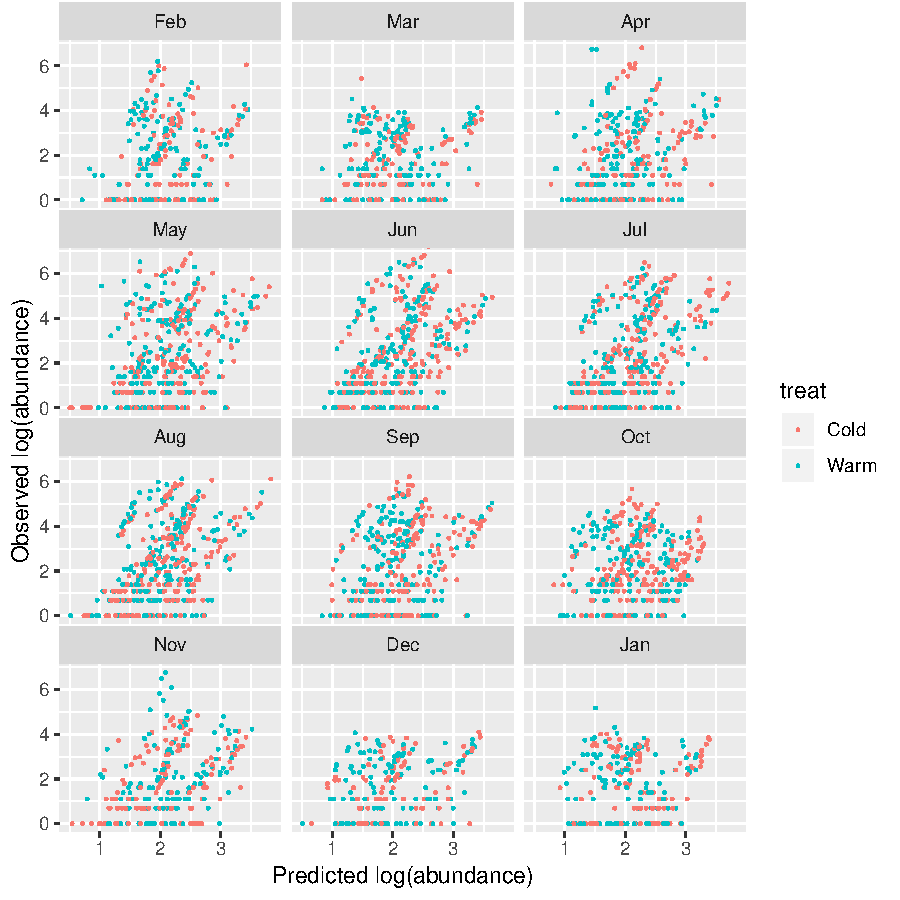
\includegraphics[scale = 0.5]{../Graph/as12op.png}
  \caption{\textbf{The observed value and predicted value of
  the allometric scaling model.}
  The red colour in graph represents samples of warming condition and the blue colour represents samples of ambient condition. }
\end{figure}

\section*{3 Plante-Downing model}
The coefficients of Plante-Downing model under different conditions were listed in figure 6. According to the observed value against predicted value of $log(abundance)$ in figure 7, Plante-Downing model fitted quite well into the model.



\begin{figure}[H]
  \centering
  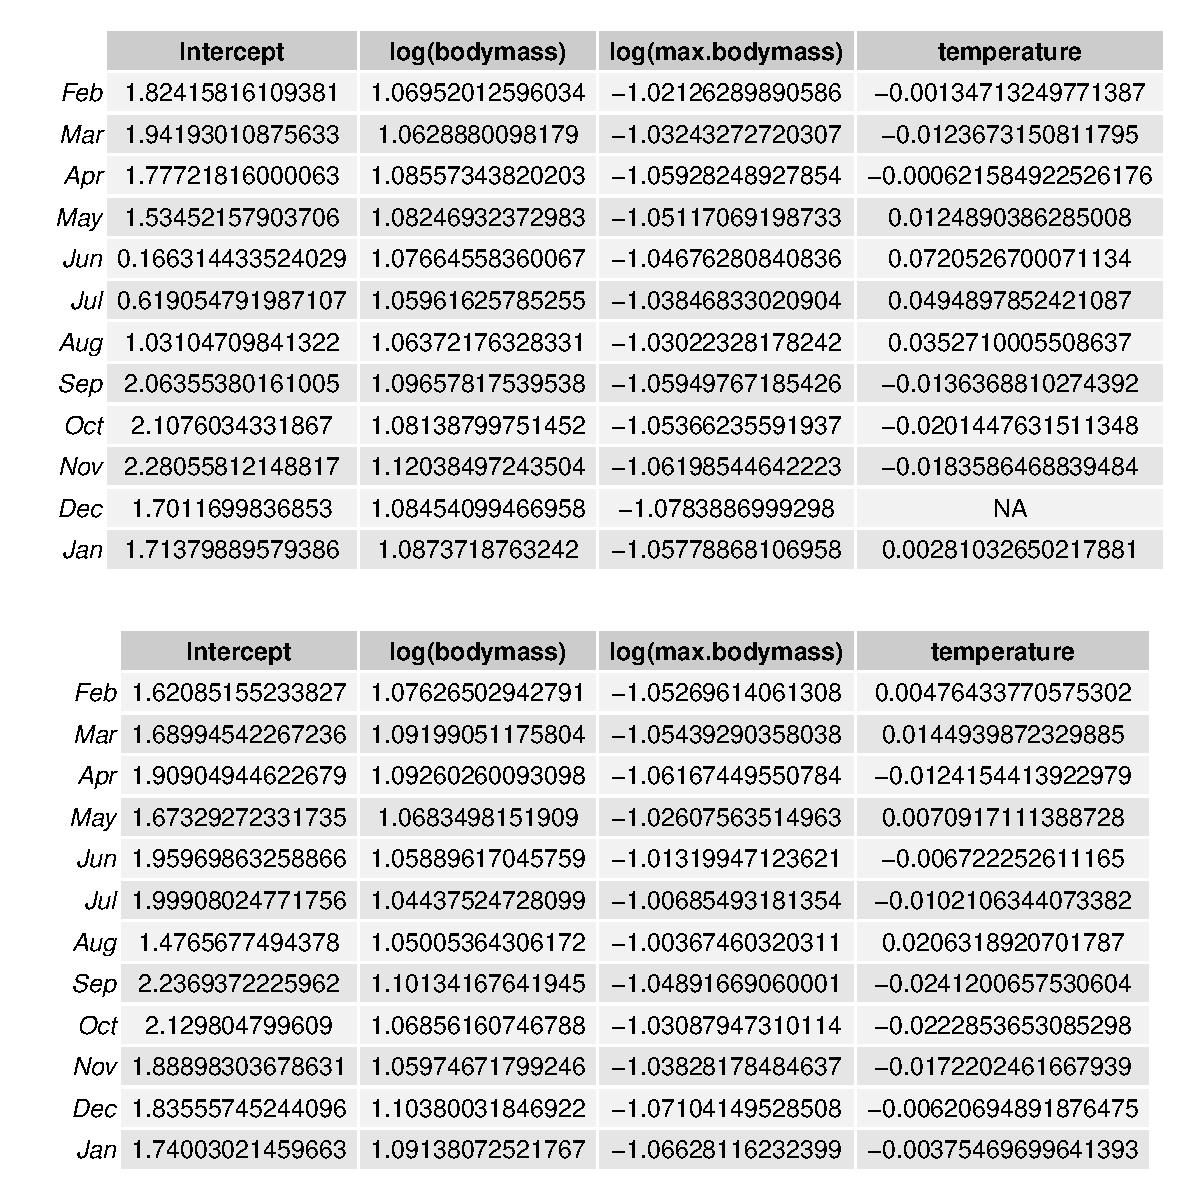
\includegraphics[scale = 0.7]{../Graph/pdcoef.png}
  \caption{\textbf{The coefficients of the Plante-Downing model.}
   The table on the top is the coefficients under warm condition. The table in the bottom is the coefficients under ambient condition. }
\end{figure}

\begin{figure}[H]
  \centering
  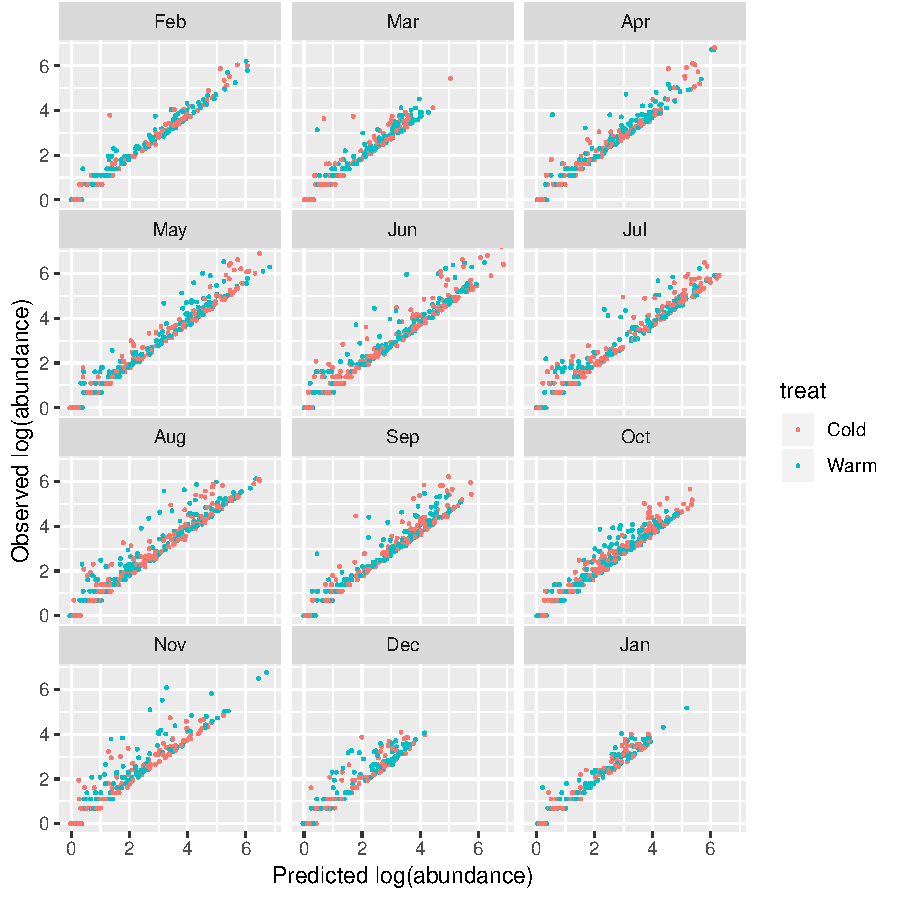
\includegraphics[scale = 0.5]{../Graph/pd12l.png}
  \caption{\textbf{The observed value and predicted value of
  the Plante-Downing model.}
  The red colour in graph represents samples of warming condition and the blue colour represents samples of ambient condition. }
\end{figure}


\section*{4 Model selection}
The AIC results of both models are shown in figure 8. Generally, the model with a relatively lower AIC is a better fitted model. Therefore, we can tell from figure 8 that Plante-Downing model is a better model to explain the relationship between abundance and bodymass in freshwater microbial communities.


\begin{figure}[H]
  \centering
  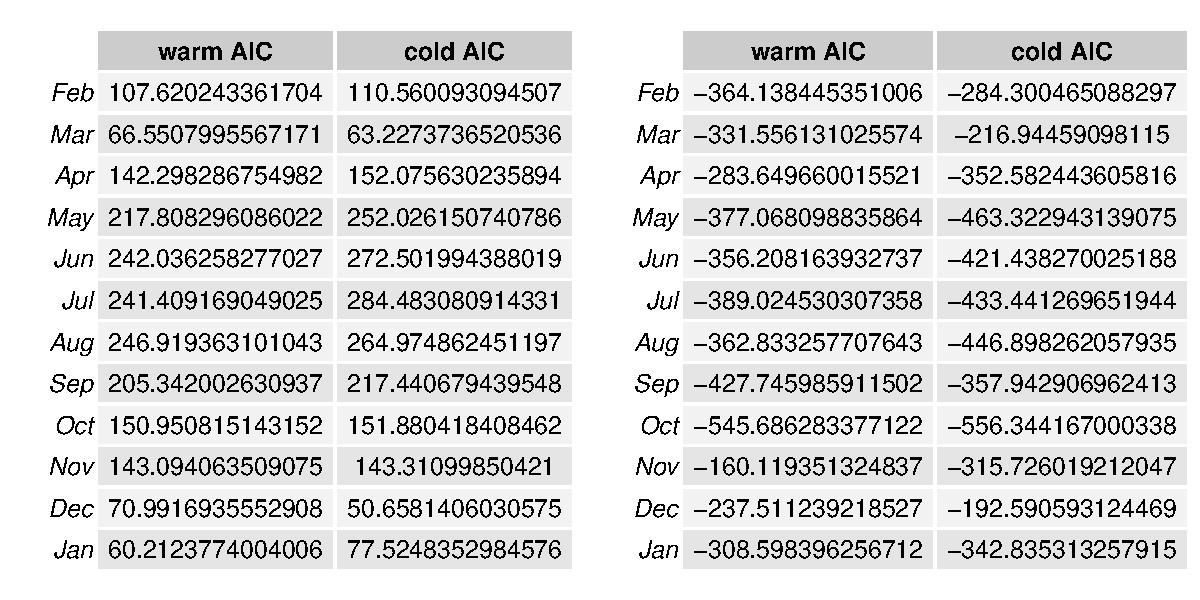
\includegraphics[scale = 0.8]{../Graph/aic.png}
  \caption{\textbf{The AIC value of the two model under both warming and ambient condition.}
  The table on the left is the AIC value of allometric scaling model.The table on the right is the AIC value of Plante-Downing model. }
\end{figure}

\section*{Discussion}
From the results of AIC, we can clearly concluded that Plante-Downing model fitted freshwater microbial communities data better than the allometric scaling model, but the widely used allometric scaling model still gave us some feedbacks.
The freshwater microbial communities under warming condition tend to have a lower growth rate in population.
The bad performance of allometric scaling model in AIC largely accounts for the small abundance in many sampled species.
We can see from figure 5 that many data points lied on the line $y= 0$, which indicated that the abundance of these sampled species in that month is 1. \\
Although the Plante-Downing model had a good performance in AIC, we need to realize that this empirical model was very likely to have a good fit to the data in this case because the biomass here is calculated by the multiplication of bodymass and abundance.
If we assinged $A$ as abundance and $B$ as bodymass, we can subsitute $\overline{B}$ with ${B}_{mean}*A$ into its formula.
Then we can discover that $ \log(A) = a +b \log({B}_{mean}*A) - c \log(\mathit{B}_{max}) + d T$.
The above formula can be transformed to $\log(A) = \log(({B}_{mean}*A)^b/\log(\mathit{B}_{max})^c) + d T + a$.
Due to the appearance of abundance on both sides of the equation, the model was very easy to have a good fit with the adjustment of constant value b and c.
For further optimizing the Plante-Downing model in this case, it is better to use projection to calculate the population of freshwater microbial communities in the following month.
In this way, the abundance of each month can be linked together.  \\
In addition, the exclusion of some abnormal data might affect the model fitting.
I excluded those abnormal data because those microbes are recorded to have a spherical shape but the length and width recorded can be quite different.
For example, the length and with of a taxa recorded to have a spherical shape is 1200 $\mu m$ and 21 $\mu m$.
However, the deletion of these data might lead to unknown effects to the model fitting.
Thoses deleted individuals might play key roles in the freshwater microbial communities like working as predator.
Next time doing such data handling, it is better to correct those abnormal data instead of deleting it.

\section*{Conclusion}
In conclusion, the Plante-Downing model performed better than the allometric scaling model in AIC. The results of this article supported Yvon's statements that freshwater microbial communities biomass decreased in warming condition. This article also validated Yvon's statement that the slope of warming condition was steeper, implicating freshwater microbial communities had a relatively lower growth rate of abundace under warming condition.



\newpage
%TC:ignore
\bibliographystyle{apalike}
\bibliography{bib.bib}
%TC:endignore

\end{linenumbers}

\end{document}\grid
\grid
